\section{Virtueller Sensorknoten}
\label{sec:arch:vsk}
Virtuelle Sensorknoten sind Sensorknoten die keine Hardware besitzen, sondern nur aus Software bestehen. Sie berechnen Messwerte nach bestimmten Verfahren, um Daten für Orten bereitzustellen an denen es nicht möglich Messungen mit physische Sensorknoten durchzuführen. 

\subsection{Gesamtüberblick}

Ein virtueller Sensorknoten ist definiert über seine Strategie, welche in einer config.json Datei beschrieben wird. Diese Config wird vom ConfigLoader ausgelesen und in Variablen für die Laufzeit geladen. Wenn die Config geladen wurde, wird der virtuelle Sensorknoten gestartet. Hierzu wird zuerst die MQTT-Verbindung aufgebaut über die die berechneten Messwerte versendet werden sollen. Anschließend wird die in den Config beschriebene Strategie ausgeführt. Ab diesem Zeitpunkt sendet der virtuelle Sensorknoten Messwerte.
Im Abschnitt \ref{strategies} werden die verschiedenen Strategien und ihre Funktionsweisen genauer beschrieben. 

\begin{figure}[H]
	\centering
	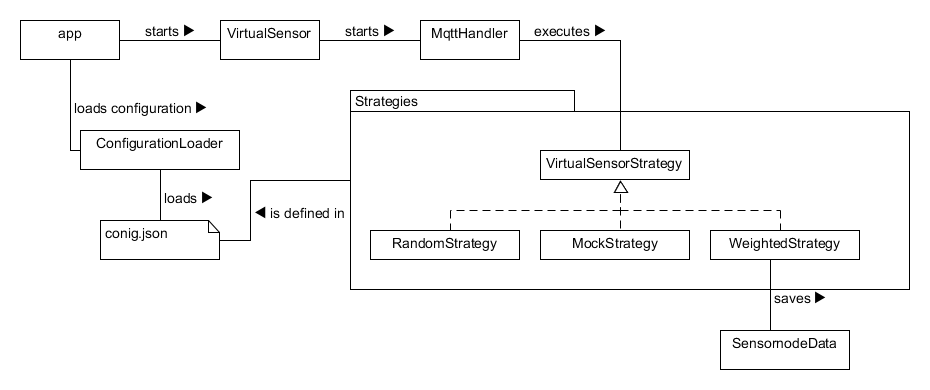
\includegraphics[width=1\linewidth]{./ressourcen/VSK-Architektur.png}
	\caption{Überblick über den Aufbau eines virtuellen Sensorknotens}
	\label{img:vsk_architetktur}
\end{figure}

\subsection{Strategien}
\label{strategies}
Die Mock-Strategie ist die einfachste Strategie. Hierbei werden die in der Config fest vorgegebene Werte für die verschiedenen Umweltfaktoren gesendet. Diese Werte müssen nicht der Realität entsprechen und dienen hauptsächlich zum Testen von anderen Komponenten, die mit diesen Daten weiterarbeiten müssen.

Die Random-Strategie ist ähnlich einfach. Sie sendet zufällige Werte aus einem vorgegebenen Intervall. In der Config Datei werden für die verschiedenen Umweltfaktoren jeweils ein minimal und ein maximal Wert angegeben. Diese Strategie ist wie die Mock-Strategie zum Testen der anderen Komponenten entwickelt worden.

Die letzte Strategie ist die Weighted-Strategie und ist die einzige Strategie, welche virtuelle Messwerte aus realen Messwerten berechnet. Über die Config können drei Sensorknoten angegeben werden, deren Messwerte in die Berechnung mit einfließen sollen. Jeder dieser Sensorknoten hat zusätzlich noch eine Gewichtung definiert, sodass z.B. weiter entfernte Sensorknoten weniger starken Einfluss auf den virtuellen Messwert haben. Durch die Gewichtung können somit verschiedenen örtliche Gegebenheiten der verschiedenen Sensorknoten berücksichtigt werden.